\subsection{Q2: Exploration 2.6.3 (Page 55)}
\label{Q2:Expl 2.6.3 SubSection}

\subsubsection{Task 2.7}
\label{Q1:Expl 2.6.3(2.7) SubSubSection}

\begin{tcolorbox}[colback=gray!20!white,colframe=gray!20!white]
  \emph{\textbf{Question 2.7 (a)} For each digit, report the number of input units where there is a weight of 1 and the input unit is also active. This should be easily visually perceptible in the display. You should find some variability in these numbers across the digits. \textbf{(b)} Why does the activation value of the receiving unit not reflect any of this variability? \textbf{(c)} What would be a better variable to examine in order to view this underlying variability, and why? [Mark: 10]}
\end{tcolorbox} 
\vspace{0.5cm}

In \cref{Q2.7A-Connected Digits} is the tabulated data record from the Emergent software. The data presented is the input data that is given to the receiving unit in the form of input patterns that display as digits from 0 to 9. In each individual digit, there are specific input data that activate it as seen in \cref{Q2.7.1} by the yellow (lit) up squares, these connect and directly relate to the receiving unit as depicted by the yellow lines. \\

The reason behind the receiving unit only activating on the number 8 digit in because all 17 input points are connected to the receiving unit whereas for the other 9 digits only up to 80\% of them are connected where the weights are easily distinguishable in \cref{Q2.7.1}. A better value to examine would be the net values of $e_{bar\_l}$ as it alters the activation value of each input unit without changing the original excitatory conductance ($e_{bar\_e}$).

\begin{table}[H]
\begin{center}
 \footnotesize
 \begin{tabular}{|c||c|c|c|}
 \hline
 \multicolumn{4}{|c|}{Number of connected and active inputs for each individual digit.} \\
 \hline \hline
 Digits & Connected& Active& Value of\\
  & (Weight of 1) & (Active Sensors)& Receiving Unit\\
 \hline \hline
 0 & 6 & 12 & 0.0000 \\\hline
 1 & 6 & 13 & 0.0000 \\\hline
 2 & 12 & 15 & 0.0000 \\\hline
 3 & 13 & 15 & 0.0000 \\\hline
 4 & 5 & 14 & 0.0000 \\\hline
 5 & 14 & 16 & 0.0000 \\\hline
 6 & 12& 15 & 0.0000 \\\hline
 7 & 6 & 11 & 0.0000 \\\hline
 8 & 17 & 17 & 0.9500 \\\hline
 9 & 12 & 15 & 0.0000 \\\hline
 \end{tabular} \\ 
 \caption{Number of connected and active inputs for each individual digit.}
 \label{Q2.7A-Connected Digits}
\end{center}
\end{table}

\begin{figure}[H]
\centering
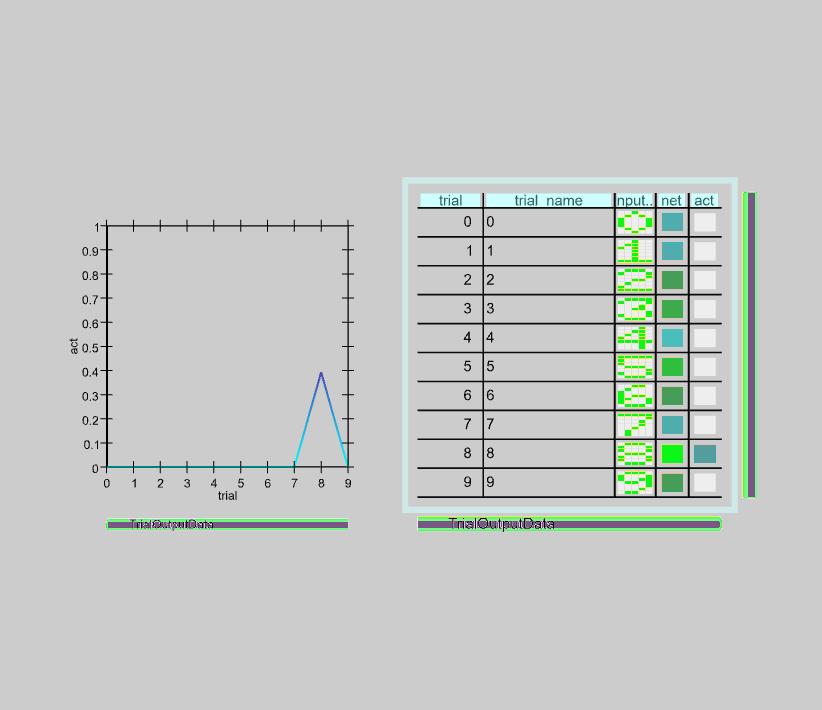
\includegraphics[scale=0.5]{Media/Main/EQ2/2.7-S0.png}
\caption{Graphical output of a full run cycle for this project.}
\label{Q2.7.0}
\end{figure}

\begin{figure}[H]
\centering
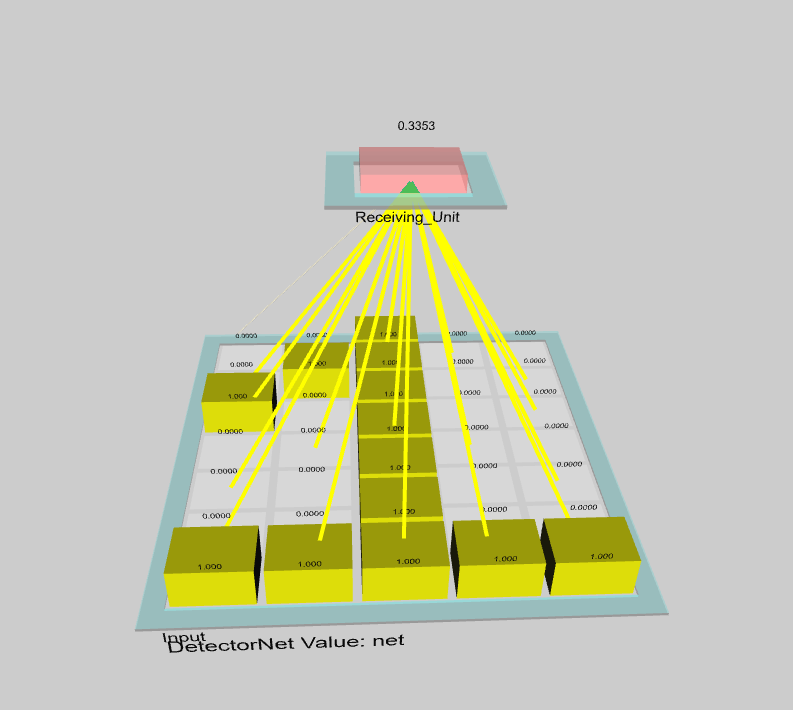
\includegraphics[scale=0.5]{Media/Main/EQ2/2.7-S1.png}
\caption{Visual representation of the connected data, input data and receiving unit.}
\label{Q2.7.1}
\end{figure}

\subsubsection{Task 2.9}
\label{Q1:Expl 2.6.3(2.9) SubSubSection}

\begin{tcolorbox}[colback=gray!20!white,colframe=gray!20!white]
  \emph{\textbf{Question 2.9 (a)} What happens to the pattern of receiving unit activity when you reduce $g_{bar\_l}$ to 6? \textbf{(b)} What happens with $g_{bar\_l}$ values of 4, 1, and 8? \textbf{(c)} Explain the effect of changing $g_{bar\_l}$ in terms of the point neuron activation function. \textbf{(d)} What might the consequences of these different response patterns have for other units that might be listening to the output of this receiving unit? Try to give some possible advantages and disadvantages for both higher and lower values of $g_{bar\_l}$. [Mark: 13]}
\end{tcolorbox} 
\vspace{0.5cm}

The default settings for the value of $g_{bar\_l}$ is 7, decreasing it to a value of 6 increases the activation value on the number 8 digit from 0.3930 to 0.9024. Changing the values of $g_{bar\_l}$ to 4, 1 and 8 are shown in \cref{Q2.9 Table} for all the digits show a direct relationship between $g_{bar\_l}$ and the receiving unit. By changing the $g_{bar\_l}$, the point neuron activation function changes in terms of the threshold and the change in $g_{bar\_l}$ changes the threshold allowing for the change in activation value. It's seen that as $g_{bar\_l}$ is decreased the activation value increases in the receiving unit and observing the value change in \cref{Q2.9 Table} and it can also been seen that the lower values of $g_{bar\_l}$ allows for the surrounding units to copy in weight and as such allows the digits to activate the receiving unit. The higher the number the more accurate the weight is and therefore the number 8 digit is the only one that can activate the receiving unit so therefore the higher the value of $g_{bar\_l}$ the more accurate the weights of the individual units.

\begin{table}[H]
\begin{center}
 \footnotesize
 \begin{tabular}{|c||c|c|c|c|c|c|c|c|c|c|}
 \hline
 \multicolumn{11}{|c|} {} \\
 $g_{bar\_l}$ & No. 0 & No.1 & No.2 & No.3 & No.4 & No.5 & No.6 & No.7 & No.8 & No.9 \\ 
 \hline \hline
 7 & 0 & 0 & 0 & 0 & 0 & 0 & 0 & 0 & 8.3930 & 0 \\\hline
 6 & 0 & 0 & 0.0033 & 0 & 0.1357 & 0 & 0 & 0 & 0.9024 & 0\\\hline
 4 & 0 & 0 & 0.9280 & 0.9478 & 0 & 0.9588 & 0.9280 & 0 & 0.9742 & 0.9280 \\\hline
 1 & 0.9842 & 0.9842 & 0.9925 & 0.9929 & 0.9788 & 0.9932 & 0.9925 & 0.9842 & 0.9938 & 0.9925 \\\hline
 8 & 0 & 0 & 0 & 0 & 0 & 0 & 0 & 0 & 0.0009 & 0 \\\hline
 \end{tabular} \\ 
 \caption{Recieving values for individual digits with different $g_{bar\_l}$ values.}
 \label{Q2.9 Table}
\end{center}
\end{table}